%%%%%%%%%%%%%%%%%%%%%%%%%%%%%%%%%%%%%%%%%
% Beamer Presentation
% LaTeX Template
% Version 1.0 (10/11/12)
%
% This template has been downloaded from:
% http://www.LaTeXTemplates.com
%
% License:
% CC BY-NC-SA 3.0 (http://creativecommons.org/licenses/by-nc-sa/3.0/)
%
%%%%%%%%%%%%%%%%%%%%%%%%%%%%%%%%%%%%%%%%%

%----------------------------------------------------------------------------------------
%	PACKAGES AND THEMES
%----------------------------------------------------------------------------------------

\documentclass{beamer}
\usepackage{xcolor}

\mode<presentation> {

% The Beamer class comes with a number of default slide themes
% which change the colors and layouts of slides. Below this is a list
% of all the themes, uncomment each in turn to see what they look like.

%\usetheme{default}
%\usetheme{AnnArbor}
%\usetheme{Antibes}
%\usetheme{Bergen}
%\usetheme{Berkeley}
%\usetheme{Berlin}
%\usetheme{Boadilla}
%\usetheme{CambridgeUS}
%\usetheme{Copenhagen}
%\usetheme{Darmstadt}
%\usetheme{Dresden}
%\usetheme{Frankfurt}
%\usetheme{Goettingen}
%\usetheme{Hannover}
%\usetheme{Ilmenau}
%\usetheme{JuanLesPins}
%\usetheme{Luebeck}
\usetheme{Madrid}
%\usetheme{Malmoe}
%\usetheme{Marburg}
%\usetheme{Montpellier}
%\usetheme{PaloAlto}
%\usetheme{Pittsburgh}
%\usetheme{Rochester}
%\usetheme{Singapore}
%\usetheme{Szeged}
%\usetheme{Warsaw}

% As well as themes, the Beamer class has a number of color themes
% for any slide theme. Uncomment each of these in turn to see how it
% changes the colors of your current slide theme.

%\usecolortheme{albatross}
%\usecolortheme{beaver}
%\usecolortheme{beetle}
%\usecolortheme{crane}
%\usecolortheme{dolphin}
%\usecolortheme{dove}
%\usecolortheme{fly}
%\usecolortheme{lily}
%\usecolortheme{orchid}
%\usecolortheme{rose}
%\usecolortheme{seagull}
%\usecolortheme{seahorse}
%\usecolortheme{whale}
%\usecolortheme{wolverine}

%\setbeamertemplate{footline} % To remove the footer line in all slides uncomment this line
%\setbeamertemplate{footline}[page number] % To replace the footer line in all slides with a simple slide count uncomment this line

%\setbeamertemplate{navigation symbols}{} % To remove the navigation symbols from the bottom of all slides uncomment this line
}

\usepackage{graphicx} % Allows including images
\usepackage{booktabs} % Allows the use of \toprule, \midrule and \bottomrule in tables

%----------------------------------------------------------------------------------------
%	TITLE PAGE
%----------------------------------------------------------------------------------------

\title[RW-HDP]{Combining random walks and nonparametric topic model for network community detection} % The short title appears at the bottom of every slide, the full title is only on the title page

\author{Ruimin Zhu} % Your name
\institute[Department of Statistics] % Your institution as it will appear on the bottom of every slide, may be shorthand to save space
{
Northwestern University \\ % Your institution for the title page
\medskip
\textit{ruiminzhu2014@u.northwestern.edu} % Your email address
}
\date{\today} % Date, can be changed to a custom date

\begin{document}

\begin{frame}
\titlepage % Print the title page as the first slide
\end{frame}

\begin{frame}
\frametitle{Outline} % Table of contents slide, comment this block out to remove it
\tableofcontents % Throughout your presentation, if you choose to use \section{} and \subsection{} commands, these will automatically be printed on this slide as an overview of your presentation
\end{frame}

%----------------------------------------------------------------------------------------
%	PRESENTATION SLIDES
%----------------------------------------------------------------------------------------

%------------------------------------------------
\section{Review of network community detection}
\begin{frame}
\frametitle{Network community detection}
\begin{itemize}
	\item matrix factorization methods
	\item optimization methods
	\item generative models
	\item other methods
\end{itemize}
\end{frame}

\section{Inspirations}
\begin{frame}
\frametitle{Where do the inspirations come from}
RW-HDP combines \textcolor{blue}{random walks} and \textcolor{blue}{topic model} for community detection.\\
\vspace{3mm}

Conducting random walks is a way of aggregating information. Each random walker is an agent who explores a local part of the network. Combining the information they collected properly, we get a big picture of the network.\\
\vspace{3mm}

Topic models are generative models that generally used for documents analysis.
\end{frame}

\subsection{random walk + deep learning}
\begin{frame}
\frametitle{Deepwalk}
\begin{columns}[t] % The "c" option specifies centered vertical alignment while the "t" option is used for top vertical alignment
	
	\column{.4\textwidth} % Left column and width
	\begin{enumerate}
		\item Conduct short random walks on the network
		\item Treat them as sentences
		\item Deep learning for word (vetex) embedding
		\item Use embedding for other tasks
	\end{enumerate}
	
	\column{.6\textwidth} % Right column and width
	\begin{figure}
		\centering
		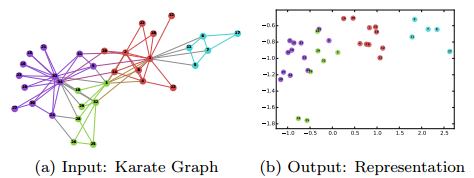
\includegraphics[scale=0.4]{deepwalk.png}
	\end{figure}
\end{columns}
\end{frame}

\subsection{SSN-LDA}
\begin{frame}
\frametitle{SSN-LDA}
...
\end{frame}


\section{RW-HDP}
\subsection{basic idea}
\begin{frame}
\frametitle{Basic idea}
\begin{enumerate}
	\item Conduct random walks on the network. Treat vertexes as words, communities as topics, and random walks as documents
	\item Use topic model to find the topic structure of each document
	\item Use Bayes theorem to find the probabilities of a vertex belonging to different topics and classify it to the largest one
\end{enumerate}
\end{frame}

\subsection{Random walks}
\begin{frame}
\frametitle{Random walks}
Let $N_d$ be the length of the $d^{th}$ random walks. The length can either be fixed or is a Poisson random variable.\\
\vspace{3mm}

Randomly sample $D$ vertexes from the network as starting points of random walks.\\
\vspace{3mm}

Conduct $D$ random walks and treat them as documents. 
\end{frame}

\subsection{HDP topic model}
\begin{frame}
\frametitle{Stick breaking construction}
...
\end{frame}

\begin{frame}
\frametitle{Graph representation}
...
\end{frame}

\subsection{Inference}
\begin{frame}
\frametitle{Conditional distributions}
Using Markov blanket we get the following conditional distributions
\begin{align*}
p(z_{dn}^i=1|\pi_d, \beta_{1:\infty},w_{dn},c_d) & \propto \exp\{\log\sigma_i(\pi_d)+\sum\limits_{k=1}^{\infty}c_{di}^k\log\beta_{k,w_{dn}}\}\\
p(c_{di}^k=1|\nu, \beta_{1:\infty},w_d, z_d) & \propto \exp\{\log\sigma_k(\nu)+\sum\limits_{n=1}^{N}\log\beta_{k,w_{dn}}\}\\
p(\pi_{di}|z_d) & \sim \text{ Beta}(1+\sum\limits_{n=1}^{N}z_{dn}^i, \alpha+\sum\limits_{n=1}^{N}\sum_{j>i}z_{dn}^j)\\
p(v_k|c) & \sim \text{ Beta}(1+\sum\limits_{d=1}^{D}\sum\limits_{i=1}^{\infty}c_{di}^k, \omega+\sum\limits_{d=1}^{D}\sum\limits_{i=1}^{\infty}\sum_{j>k}c_{di}^j)\\
p(\beta_k|z,c,w) & \sim \text{ Dirichlet}(\eta+\sum\limits_{d=1}^{D}\sum\limits_{i=1}^{\infty}c_{di}^k\sum\limits_{n=1}^{N}z_{dn}^iw_{dn}).
\end{align*}
Notice that all of them are in Exponential families.
\end{frame}

\begin{frame}
\frametitle{Stochastic variational inference}
Based on the conditional distributions, we using the following variational family under the mean field assumption
\begin{align*}
q(\beta,\nu,z,\pi)  = & \Big(\prod_{k=1}^{K}q(\beta_k|\lambda_k)q(\nu_k|a_k)\Big)\times\\
&\Big(\prod_{d=1}^{D}\prod_{i=1}^{T}q(c_{di}|\zeta_{di})q(\pi_{di}|\gamma_{di})\prod_{n=1}^{N}q(z_{dn}|\phi_{dn})\Big)
\end{align*}

The latent variables $c_{di}, \pi_{di}, z_{dn}$ depends only on a single document, while the global variables $v_k, \beta_k$ depends on all documents. To efficiently update the proxy, we can use \textcolor{blue}{Stochastic Variational Inference} method.
\end{frame}

\subsection{Community assignment}
\begin{frame}
\frametitle{Bayes theorem for community assignment}
...
\end{frame}

\section{Experiments}
\subsection{data sets}
\subsection{evaluation metrics}
\subsection{comparison models}
\subsection{results}
\subsection{Pros and Cons}
\begin{frame}
\frametitle{Pros and Cons}
\begin{columns}[t] % The "c" option specifies centered vertical alignment while the "t" option is used for top vertical alignment
	
	\column{.5\textwidth} % Left column and width
	Pros
	\begin{enumerate}
		\item Nonparametric topic model allow community number auto detection
		\item Soft-clustering 
		\item High accuracy compared to other generative models
		\item Can be extended to online setting
	\end{enumerate}
	
	\column{.5\textwidth} % Right column and width
	Cons
	\begin{enumerate}
		\item The inference of probabilistic model is always slow, even SVI is used
	\end{enumerate}
\end{columns}
\end{frame}



\section{Future works}
\begin{frame}
\frametitle{Future works}
\begin{enumerate}
	\item Include teleportation to allow single agent to explore a larger area of the network
	\item Hyperparameters tuning
	\item Ground truth benchmarks comparison
\end{enumerate}
\end{frame}

\section{References}
\begin{frame}
\frametitle{References}
...
\end{frame}
\end{document}

\begin{frame}
	\Huge{\centerline{Thank You}}
\end{frame}


\begin{columns}[t] % The "c" option specifies centered vertical alignment while the "t" option is used for top vertical alignment
	
	\column{.5\textwidth} % Left column and width
	Stochastic Methods
	
	\begin{enumerate}
		\item Gibbs Sampling
		\item Metropolis-Hasting Algorithm
	\end{enumerate}
	
	\column{.5\textwidth} % Right column and width
	Deterministic Methods
	\begin{enumerate}
		\item Laplace Approximation
		\item Variational Inference
	\end{enumerate}
\end{columns}